\documentclass[oneside, final, 14pt]{extarticle}
\usepackage[utf8]{inputenc}
\usepackage[T2A]{fontenc}
\usepackage[english, russian]{babel}
\usepackage{vmargin}
\setpapersize{A4}
\setmarginsrb{2cm}{1.5cm}{1cm}{1.5cm}{0pt}{0mm}{0pt}{13mm}
\usepackage{indentfirst}
\sloppy
\usepackage{graphicx}
\usepackage{amsmath}
\usepackage{titlesec}
\usepackage{hyperref}
\usepackage{adjustbox}
\usepackage{tabularx}
\usepackage{array}
\usepackage{tikz}
\usetikzlibrary{arrows.meta, positioning, shapes}

\graphicspath{{./images/}}

\usepackage[backend=bibtex]{biblatex}
\addbibresource{bibliography.bib}

\def\verbatimtabsize{4\relax}

\begin{document}

\begin{titlepage}
  \centerline{Министерство науки и высшего образования Российской Федерации}
  \medskip
  \centerline{ФЕДЕРАЛЬНОЕ ГОСУДАРСТВЕННОЕ АВТОНОМНОЕ ОБРАЗОВАТЕЛЬНОЕ}
  \medskip
  \centerline{УЧРЕЖДЕНИЕ ВЫСШЕГО ОБРАЗОВАНИЯ}
  \medskip
  \centerline{"<Национальный исследовательский университет ИТМО">}
  \vfill
  \centerline{Факультет информационных технологий и программирования}
  \medskip
  \centerline{Кафедра Речевых информационных систем}
  \vfill
  \vfill
  \centerline{Отчёт по курсовой работе}
  \vfill
  \centerline{Научно исследовательская работа по теме:}
  \medskip
  \centerline{"<Разработка безэталонного метода объективной оценки индекса разборчивости речи">}
  \vfill
  \null \hfill
  \begin{minipage}{0.4\textwidth}
    Выполнил студент гр.\,M4121:
	\par
	\medskip
	Давыдов~Д.\,А.\,
	\rule{3.5cm}{0.25pt}
	\par
	\medskip
	Руководитель:
	\par
	\medskip
	Столбов~М.\,Б.\,
	\rule{3.5cm}{0.25pt}
  \end{minipage}
  \vfill
  \centerline{г.~Санкт-Петербург}
  \centerline{2025 год}
\end{titlepage}
\setcounter{page}{2}

\tableofcontents

\newpage
\section*{Введение}

Разборчивость речи является критически важным параметром для профессиональных дикторов, определяющим эффективность передачи информации аудитории. В настоящее время для оценки разборчивости речи применяются как субъективные, так и объективные методы.

Субъективные методы, такие как экспертные оценки или тестирование на группах слушателей, обладают высокой точностью, но требуют значительных временных и организационных затрат. Объективные методы, включая алгоритмические и инструментальные подходы, позволяют автоматизировать процесс оценки, однако часто зависят от эталонных данных и не всегда учитывают специфику профессиональной дикторской речи.

Учитывая недостатки существующих подходов, актуальной задачей является разработка специализированного метода оценки разборчивости речи, адаптированного именно для дикторов. \textbf{Целью данного исследования} является создание \textbf{безэталонного метода оценки разборчивости речи}, который позволит объективно и эффективно анализировать качество произношения дикторов в различных условиях без необходимости использования эталонных записей. Такой подход упростит процесс оценки и сделает его более доступным для применения в профессиональной среде.

\textbf{Задачи исследования:}
\begin{enumerate}
\item Анализ существующих субъективных и объективных методов оценки разборчивости речи (РР) и выявление их ограничений применительно к дикторской речи.
\item Исследование возможностей применения нейросетевых моделей для безэталонной оценки РР с учётом специфики профессионального дикторского произношения.
\item Разработка архитектуры нейронной сети, способной оценивать РР без использования эталонных речевых образцов.
\item Экспериментальная проверка точности и устойчивости предложенного метода на корпусе дикторских записей в различных акустических условиях.
\item Сравнение эффективности разработанного метода с традиционными подходами к оценке РР.
\end{enumerate}

\textbf{Объект исследования} -- разборчивость речи профессиональных дикторов как ключевая характеристика качества устной коммуникации. В работе рассматриваются акустические и лингвистические особенности дикторской речи, влияющие на её восприятие, а также технические аспекты автоматизированной оценки этого параметра.

\textbf{Предмет исследования} -- методы и алгоритмы безэталонной оценки разборчивости речи на основе нейросетевых технологий. Особое внимание уделяется возможностям глубокого обучения для выявления и количественного измерения параметров РР без сравнения с эталонными образцами.

\textbf{Исследование сосредоточено} на разработке нейросетевого подхода к оценке РР, не требующего эталонных записей для анализа качества дикторской речи. Основной акцент делается на создании системы, способной адаптироваться к различным стилям профессионального произношения и условиям записи.

\newpage

\section{Теоретические основы разборчивости речи}

Оценка разборчивости речи является ключевой задачей во многих областях, включая телекоммуникации, аудио-криминалистику и разработку слуховых аппаратов. Понимание того, насколько хорошо слушатель может разобрать произнесенные слова конкретного диктора в различных акустических условиях, позволяет не только оценивать качество систем связи, но и разрабатывать новые методы обработки сигналов, направленные на улучшение восприятия речи. В реальных условиях речевой сигнал часто подвергается искажениям из-за фонового шума и реверберации, что делает задачу оценки разборчивости особенно актуальной. В данном разделе будут рассмотрены фундаментальные концепции разборчивости речи, факторы, оказывающие на нее влияние, а также существующие методы ее объективной и субъективной оценки.

\subsection{Понятие разборчивости речи}

Разборчивость речи определяется как доля речевого сигнала, содержание которого может быть правильно распознано слушателем \cite{Sharma2016}. Этот показатель является важным количественным параметром для множества приложений. Например, в сфере телекоммуникаций качество канала связи может оцениваться по его влиянию на разборчивость речи \cite{Steeneken1980}. В области разработки слуховых аппаратов разборчивость служит метрикой их эффективности \cite{vanHoesel2003}, а в акустике помещений она помогает определить влияние архитектурных особенностей на восприятие речи \cite{Houtgast1985}.

Оценка разборчивости традиционно проводится с помощью субъективных тестов, в ходе которых испытуемые прослушивают речевые образцы и выполняют определенную лингвистическую задачу. Задачи могут варьироваться от распознавания бессмысленных слогов \cite{Miller1955} до идентификации ключевых слов в предложениях \cite{Kalikow1977}. Наиболее распространенным субъективным методом является оценка по абсолютной категориальной шкале (ACR), где слушатели оценивают качество по шкале от 1 (плохо) до 5 (отлично). Усредненная оценка по группе слушателей называется средней экспертной оценкой (Mean Opinion Score, MOS) \cite{Zha2003}. MOS считается наиболее надежным показателем качества и разборчивости, однако его получение сопряжено со значительными трудностями: необходимо привлекать большое количество слушателей для минимизации субъективной предвзятости, контролировать акустические условия прослушивания и используемое оборудование, что делает процесс дорогостоящим и трудоемким \cite{Agrawal2025}. Это особенно усложняет масштабирование оценки для больших объемов данных или для низкоресурсных языков.

\subsection{Факторы, влияющие на разборчивость речи}

На разборчивость речи диктора в реальных условиях влияет множество факторов, искажающих исходный речевой сигнал. В рамках данной работы основное внимание уделяется аддитивному шуму и реверберации.

\textbf{Аддитивный шум} является одной из самых распространенных причин ухудшения разборчивости. Это может быть как стационарный шум (например, гул компьютерного оборудования или вентиляции), так и нестационарный (например, уличный шум). Наличие шума маскирует полезный речевой сигнал, затрудняя его восприятие \cite{Sharma2016}. Уровень влияния шума на разборчивость принято характеризовать отношением сигнал/шум (Signal-to-Noise Ratio, SNR).

\textbf{Реверберация} возникает в замкнутых пространствах из-за многократных отражений звука от поверхностей. Ранние отражения, приходящие к слушателю вскоре после прямого звука, могут изменять тембр сигнала (эффект окрашивания), в то время как поздние отражения вызывают временное "смазывание" звука (temporal smearing), что существенно снижает разборчивость \cite{Falk2010}. Эффект реверберации зависит от геометрии помещения и звукопоглощающих свойств его поверхностей. Большинство систем обработки речи обучаются на синтетических данных, записанных в безэховых (anechoic) условиях, что создает разрыв (domain gap) с реальными акустическими средами, где всегда присутствует реверберация \cite{Wang2024}.

Для борьбы с этими факторами применяются различные алгоритмы обработки речи, такие как шумоподавление и дереверберация. Однако сами эти алгоритмы могут вносить в сигнал нежелательные артефакты, что также требует тщательной оценки итоговой разборчивости \cite{Falk2010, Vincent2006}.

\subsection{Методы оценки разборчивости речи}

Методы оценки разборчивости речи можно разделить на две большие категории: субъективные и объективные. Подробный анализ конкретных алгоритмов объективной оценки будет представлен в Разделе 2.

\textbf{Субъективные методы}, такие как тесты на основе MOS, являются <<золотым стандартом>>, но, как уже отмечалось, они дороги, медленны и не подходят для оценки в реальном времени \cite{Zha2003, Agrawal2025}.

\textbf{Объективные методы} используют алгоритмы для оценки разборчивости без участия человека. Они стремятся предсказать субъективное восприятие качества и разборчивости. Эти методы, в свою очередь, делятся на эталонные (intrusive) и безэталонные (non-intrusive).

\begin{itemize}
    \item \textbf{Эталонные методы} требуют наличия исходного, "чистого" речевого сигнала в качестве эталона для сравнения с обработанным или искаженным сигналом. К ним относятся такие стандарты, как PESQ (Perceptual Evaluation of Speech Quality) \cite{ITU-T2001} для оценки качества и STOI (Short-Time Objective Intelligibility) \cite{Taal2011} для оценки разборчивости. Подробное описание эталонных методов будет представлено в разделе 2.1.
    
    \item \textbf{Безэталонные методы} работают только с искаженным сигналом, не требуя доступа к оригиналу. Это делает их применимыми в реальных условиях, что и является целью данной работы. Примером такого подхода является алгоритм NISA (Non-Intrusive Speech Assessment) \cite{Sharma2016}. Современные подходы также используют глубокие нейронные сети для предсказания субъективного качества без эталонного сигнала \cite{Agrawal2025}. Более детальный обзор безэталонных методов будет дан в разделе 2.2.
\end{itemize}

Разработка эффективных безэталонных методов является актуальной задачей, поскольку они открывают возможности для автоматического мониторинга и оптимизации производительности систем обработки и улучшения качества речи в режиме реального времени.

\newpage

\section{Обзор существующих методов}

Методы оценки разборчивости речи исторически делятся на две основные категории: субъективные и объективные. Субъективные методы основаны на прослушивании и оценке речи людьми, в то время как объективные используют математические алгоритмы для предсказания воспринимаемого качества и разборчивости. Объективные методы, в свою очередь, подразделяются на эталонные, требующие наличия <<чистого>> исходного сигнала, и безэталонные, работающие только с искаженным сигналом.

\subsection{Эталонные методы}

Эталонные (intrusive) методы оценки качества и разборчивости речи требуют наличия двух сигналов: исходного (чистого, reference) и обработанного (искаженного, degraded). Путем их сравнения вычисляется метрика, отражающая степень искажения.

Одним из самых ранних и широко известных подходов является вычисление отношения сигнал/шум (Signal-to-Noise Ratio, SNR) и его модификаций, таких как сегментарный SNR (segSNR) \cite{DiPersia2007}. Однако эти метрики, основанные на простом сопоставлении формы волны, плохо коррелируют с субъективным восприятием, поскольку не учитывают психоакустические особенности слуха.

Более продвинутые эталонные методы основаны на моделях человеческого слуха. Ярким примером является стандарт ITU-T P.862, известный как PESQ (Perceptual Evaluation of Speech Quality) \cite{Sharma2016, Zha2005}. Алгоритм PESQ преобразует оба сигнала (исходный и искаженный) в психоакустическое представление, учитывая неравномерную чувствительность слуха к разным частотам и уровням громкости, а затем вычисляет разницу между этими представлениями. PESQ хорошо зарекомендовал себя для оценки искажений, вносимых кодеками и сетями передачи данных, и его оценки сильно коррелируют с субъективными MOS-оценками для этих типов искажений \cite{Sharma2016}.

Для оценки именно разборчивости, а не общего качества, был разработан метод \textbf{STOI (Short-Time Objective Intelligibility)} \cite{Taal2011}. STOI вычисляет корреляцию между временными огибающими коротких сегментов чистого и искаженного сигналов в разных частотных диапазонах. Этот метод показал высокую корреляцию с субъективными тестами на разборчивость речи в условиях аддитивного шума и после применения алгоритмов шумоподавления \cite{Sharma2016}.

Для более детального анализа искажений, особенно в задачах улучшения и разделения речи, были предложены метрики, основанные на декомпозиции сигнала. Например, в работе \cite{Vincent2006} оцениваемый сигнал $\hat{s}$ раскладывается на четыре компонента: целевой сигнал ($s_{target}$), ошибку интерференции ($e_{interf}$), ошибку аддитивного шума ($e_{noise}$) и ошибку артефактов ($e_{artif}$). На основе этой декомпозиции рассчитываются такие метрики, как \textbf{SDR (Signal-to-Distortion Ratio)}, \textbf{SIR (Signal-to-Interference Ratio)} и \textbf{SAR (Signal-to-Artifacts Ratio)}. Такой подход позволяет раздельно оценивать способность алгоритма подавлять помехи, шум и минимизировать вносимые им артефакты \cite{Vincent2006}.

Основным недостатком всех эталонных методов является требование наличия чистого исходного сигнала, который в большинстве реальных приложений недоступен.

\subsection{Безэталонные методы}

Безэталонные (non-intrusive) методы оценивают качество или разборчивость речи, анализируя только сам искаженный сигнал. Это делает их применимыми для мониторинга в реальном времени, что является целью данной курсовой работы.

Ранние безэталонные методы, такие как стандарт \textbf{ITU-T P.563}, использовали набор эвристических признаков, извлеченных из речевого потока, для предсказания MOS \cite{Sharma2016}. Такие признаки могли включать параметры голосового тракта, неестественные паузы, роботизированность голоса и другие аномалии.

С развитием машинного обучения появились более сложные подходы. Например, в работах \cite{Falk2004, Zha2005} предлагается извлекать большое количество перцептивных признаков, а затем использовать методы интеллектуального анализа данных (data mining), такие как деревья классификации и регрессии (CART), для выбора наиболее значимых признаков и построения модели, предсказывающей MOS.

Современные безэталонные методы активно используют глубокие нейронные сети. Эти модели обучаются на огромных базах данных, где каждый речевой семпл имеет соответствующую ему субъективную оценку (MOS). Модель учится сопоставлять акустические характеристики сигнала с его субъективным качеством. Примером такого подхода является модель \textbf{NISA (Non-Intrusive Speech Assessment)}, которая использует комбинацию извлечения признаков и регрессии на основе деревьев для оценки как качества (предсказание PESQ), так и разборчивости (предсказание STOI) \cite{Sharma2016}. Другие современные системы, такие как \textbf{SALF-MOS}, используют архитектуры на основе сверточных сетей для извлечения латентных признаков из аудио и предсказания MOS, демонстрируя высокую обобщающую способность на разных дикторах и наборах данных \cite{Agrawal2025}.

В контексте реверберации были предложены специализированные безэталонные метрики. Например, \cite{Falk2010} исследует модуляционное спектральное представление сигнала для оценки качества и разборчивости реверберированной речи. Метод, названный \textbf{SRMR (Speech-to-Reverberation Modulation Energy Ratio)}, анализирует соотношение энергий в низко- и высокочастотных областях модуляционного спектра, что позволяет оценить степень реверберации.

Ключевым преимуществом безэталонных методов является их практичность. Однако их точность сильно зависит от качества и разнообразия данных, на которых они обучались. Создание надежного безэталонного метода, который хорошо обобщается на разные типы искажений, дикторов и акустические условия, остается актуальной исследовательской задачей.

\newpage
\section{Разработка нейро-сетевого метода предсказания разборчивости речи}

Оценка разборчивости речи является важной задачей в области обработки звука и речевых технологий. Традиционные метрики, такие как STOI (Short-Time Objective Intelligibility), хотя и обеспечивают объективную оценку, требуют наличия эталонного сигнала, что ограничивает их применение в реальных условиях. В данной работе предлагается нейро-сетевой подход, позволяющий предсказывать разборчивость речи без необходимости использования эталонного сигнала, что расширяет область применения системы.

В качестве основы для обучения модели используется корпус аудиозаписей речи, искусственно искаженных с помощью аддитивного гауссовского белого шума (АГБШ) и реверберации. На этих данных модель обучается предсказывать значения STOI, что позволяет в дальнейшем оценивать разборчивость речи в условиях, когда эталонный сигнал недоступен. Такой подход сочетает преимущества объективных метрик с гибкостью нейронных сетей, адаптирующихся к различным акустическим условиям.

\subsection{Архитектура нейронной сети}

Разработанная архитектура нейронной сети представляет собой глубокую сверточную модель, специально оптимизированную для обработки мел-спектрограмм и предсказания индекса разборчивости речи STOI. Как показано на рис. \ref{fig:nn_architecture}, модель имеет последовательную структуру, состоящую из четырех сверточных блоков для извлечения признаков и трех полносвязных слоев для регрессии.

\begin{figure}[]
\centering
\begin{tikzpicture}[
    node distance=1.0cm and 0.6cm,
    layer/.style={draw, rectangle, minimum width=4cm, minimum height=0.8cm, rounded corners=3pt, align=center},
    block/.style={draw, rectangle, minimum width=4cm, minimum height=1.2cm, rounded corners=5pt, align=center, fill=blue!10},
    arrow/.style={-Stealth, thick},
    label/.style={font=\footnotesize}
]

% Вход
\node[block, fill=green!10] (input) {Input \\ Mel-spectrogram};

% Conv Blocks
\node[block, below=of input] (conv_block1) {
    Свёрточный слой \\
    BatchNorm2d(16) \\
    ReLU \\
    MaxPool2d
};
\node[block, below=of conv_block1] (conv_block2) {
    Свёрточный слой \\
    BatchNorm2d(32) \\
    ReLU \\
    MaxPool2d
};
\node[block, below=of conv_block2] (conv_block3) {
    Свёрточный слой \\
    BatchNorm2d(64) \\
    ReLU \\
    MaxPool2d
};
\node[block, below=of conv_block3] (conv_block4) {
    Свёрточный слой \\
    BatchNorm2d(128) \\
    ReLU \\
    MaxPool2d
};

% Flatten
\node[layer, fill=red!10, below=of conv_block4] (flatten) {Flatten};

% FC Layers
\node[layer, fill=purple!10, below=of flatten] (fc1) {Linear(5632, 256) \\ ReLU \\ Dropout(0.5)};
\node[layer, fill=purple!10, below=of fc1] (fc2) {Linear(256, 64) \\ ReLU \\ Dropout(0.3)};
\node[layer, fill=orange!10, below=of fc2] (output) {Linear(64, 1)};

% Стрелки
\foreach \i/\j in {input/conv_block1, conv_block1/conv_block2, conv_block2/conv_block3, 
                  conv_block3/conv_block4, conv_block4/flatten, flatten/fc1, fc1/fc2, fc2/output}
    \draw[arrow] (\i) -- (\j);

% Подписи справа
\node[right=0.5cm of output, label, align=left] {Выход: предсказание \\ STOI [0,1]};

\end{tikzpicture}
\caption{Архитектура нейронной сети для предсказания разборчивости речи}
\label{fig:nn_architecture}
\end{figure}


Входной слой модели принимает одноканальные мел-спектрограммы размерностью H×W, где H соответствует количеству мел-фильтров (64 в нашем случае), а W - количеству временных отсчетов, которое варьируется в зависимости от длины аудиозаписи. Перед подачей на вход спектрограммы нормализуются путем вычитания среднего и деления на стандартное отклонение, вычисленные по тренировочному набору данных.

Каждый из четырех сверточных блоков выполняет последовательную обработку данных. Первый слой в блоке - двумерная свертка с ядром 3×3, что позволяет сохранять пространственные размерности входного тензора. Размерность пространства признаков последовательно увеличивается от 16 в первом блоке до 128 в четвертом. За сверточным слоем следует операция пакетной нормализации (BatchNorm2d), которая стабилизирует распределение активаций и ускоряет процесс обучения. Активационная функция ReLU (Rectified Linear Unit) добавляет нелинейность в модель. Завершает каждый блок операция макс-пулинга с ядром 2×2, уменьшающая пространственные размерности в два раза.

После сверточных слоев тензор признатов преобразуется в одномерный вектор операцией выравнивания (Flatten). Размерность полученного вектора составляет 5632 элемента, что было определено экспериментальным путем на этапе проектирования архитектуры. Этот вектор служит входом для каскада полносвязных слоев.

Первый полносвязный слой (Linear) уменьшает размерность с 5632 до 256 нейронов. Для борьбы с переобучением после этого слоя применяется операция Dropout с вероятностью 0.5, случайным образом обнуляющая 50\% активаций во время обучения. Второй полносвязный слой дополнительно сокращает размерность до 64 нейронов с Dropout 0.3. Оба слоя используют активацию ReLU для введения нелинейности.

Выходной слой модели состоит из одного нейрона с линейной активацией, который предсказывает значение STOI в диапазоне от 0 до 1. В отличие от скрытых слоев, на выходе не применяется функция активации Sigmoid.

Особенностью данной архитектуры является постепенное увеличение глубины признаков (от 16 до 128 каналов) при одновременном уменьшении пространственных размерностей спектрограммы. Такой подход позволяет модели последовательно извлекать признаки разного уровня абстракции - от локальных спектральных особенностей на ранних слоях до глобальных временных паттернов на глубоких слоях. Использование пакетной нормализации после каждого сверточного слоя стабилизирует распределение активаций и позволяет использовать более высокие скорости обучения.

\subsection{Подготовка и аугментация данных}

Формирование датасета для обучения модели оценки разборчивости речи осуществлялось на основе комплексной обработки исходных аудиозаписей из базы данных CMU-MOSEI. Для обеспечения разнообразия акустических условий были применены методики искусственного искажения речевых сигналов, что позволило создать обширную коллекцию данных с контролируемыми параметрами качества.

\begin{figure}[]
	\centering
	\includegraphics[width=1\linewidth]{processing_types_distribution.png}
	\caption{Распределение типов обработки сигналов в датасете}
	\label{fig:processing_types}
\end{figure}

Как видно из Рис.~\ref{fig:processing_types}, датасет содержит три основных категории обработки сигналов: чистые записи после VAD-обработки (около 15\% данных), записи с добавленным шумом (60\%) и записи с искусственной реверберацией (25\%). Такой баланс обеспечивает достаточное разнообразие акустических условий для обучения устойчивой модели.

Предварительная обработка включала несколько критически важных этапов. Первоначально применялся энергетический метод детектирования речевой активности (VAD), вычисляемым по формуле:

\begin{equation}
	E_{dB} = 10\log_{10}\left(\frac{1}{N}\sum_{n=0}^{N-1}|x[n]|^2\right)
\end{equation}

где $x[n]$ представляет дискретные отсчеты сигнала, а $N=2048$ определяет размер анализируемого фрейма. После выделения речевых участков каждый сигнал нормализовался по амплитуде и приводился к стандартной длительности 3 секунды, что обеспечивало единообразие входных данных для нейронной сети.

\begin{figure}[h]
	\centering
	\includegraphics[width=1\linewidth]{stoi_distribution.png}
	\caption{Распределение значений STOI в датасете}
	\label{fig:stoi_dist}
\end{figure}

Анализ распределения значений STOI (Рис.~\ref{fig:stoi_dist}) показывает, что датасет охватывает весь возможный диапазон разборчивости от 0 до 1 с пиками в области высоких значений (0.8-1.0), что соответствует естественному распределению качества речи в реальных условиях. Для обеспечения баланса было применено контролируемое дублирование примеров с экстремальными значениями STOI.

Методика генерации искаженных версий включала два основных подхода. Добавление аддитивного гауссовского белого шума осуществлялось с варьируемым уровнем SNR (0-30 дБ), рассчитываемым как:

\begin{equation}
	\text{SNR} = 10\log_{10}\left(\frac{P_{\text{signal}}}{P_{\text{noise}}}\right)
\end{equation}

\begin{figure}[]
	\centering
	\includegraphics[width=1\linewidth]{stoi_vs_snr.png}
	\caption{Зависимость STOI от уровня SNR}
	\label{fig:stoi_snr}
\end{figure}

Как демонстрирует Рис.~\ref{fig:stoi_snr}, существует четкая нелинейная зависимость между уровнем SNR и значением STOI, причем наиболее значительное ухудшение разборчивости наблюдается при SNR ниже 10 дБ. Это соотношение было учтено при формировании датасета для обеспечения адекватного представления всех уровней разборчивости.

Моделирование реверберации выполнялось с использованием импульсных откликов, параметризуемых временем реверберации RT60:

\begin{equation}
	h(t) = e^{-\frac{t}{\tau}}\cdot n(t), \quad \tau = \frac{\text{RT60}}{6\ln10}
\end{equation}

где $n(t)$ представляет гауссовский случайный процесс. Параметры реверберации варьировались в диапазоне RT60 от 0.3 до 1.5 секунд, что охватывает типичные акустические условия от небольших помещений до крупных залов.

\begin{figure}[]
	\centering
	\includegraphics[width=1\linewidth]{stoi_by_processing_type.png}
	\caption{Распределение STOI по типам обработки сигналов}
	\label{fig:stoi_by_type}
\end{figure}

Анализ распределения STOI по типам обработки (Рис.~\ref{fig:stoi_by_type}) показывает, что наиболее значительное снижение разборчивости вызывают комбинированные искажения (шум+реверберация), тогда как отдельные виды обработки приводят к менее выраженному ухудшению STOI. Это наблюдение подтверждает важность включения в датасет сложных комбинированных случаев.

Расчет индекса STOI выполнялся по алгоритму:

\begin{equation}
	\text{STOI} = \frac{1}{MN}\sum_{m=1}^{M}\sum_{n=1}^{N}\frac{\text{cov}(X_{mn},Y_{mn})}{\sigma_{X_{mn}}\sigma_{Y_{mn}}}
\end{equation}

где $X(t,f)$ и $Y(t,f)$ представляют временно-частотные характеристики чистого и искаженного сигналов соответственно, $M$ - количество частотных полос, $N$ - количество временных сегментов, а $\text{cov}$ обозначает выборочную ковариацию.

Итоговый датасет содержал около 60,000 записей, каждая из которых включала:
\begin{itemize}
	\setlength{\itemsep}{0pt}
	\item Мел-спектрограмму размерностью 64×T (64 мел-фильтра)
	\item Соответствующее значение STOI
	\item Метод обработки сигнала
	\item Параметры искажений (SNR, RT60)
\end{itemize}


Такой комплексный подход к формированию данных обеспечил репрезентативное покрытие различных акустических условий и создал прочную основу для обучения точной и устойчивой модели оценки разборчивости речи. Особое внимание было уделено балансировке датасета по типам искажений и уровням разборчивости, что подтверждается представленными распределениями.

\subsection{Обучение и валидация модели}

Процесс обучения нейронной сети для предсказания индекса разборчивости речи осуществлялся в течение 50 эпох с использованием оптимизатора Adam, параметры которого ($\beta_1=0.9$, $\beta_2=0.999$) были выбраны на основе общепринятых рекомендаций для задач глубокого обучения. В качестве функции потерь применялась среднеквадратичная ошибка (MSE), вычисляемая по формуле:

\begin{equation}
\mathcal{L}_{MSE} = \frac{1}{N}\sum_{i=1}^N(y_i - \hat{y}_i)^2
\end{equation}

где $y_i$ - истинное значение STOI, $\hat{y}_i$ - предсказанное значение, $N$ - количество образцов в батче.

\begin{figure}[]
\centering
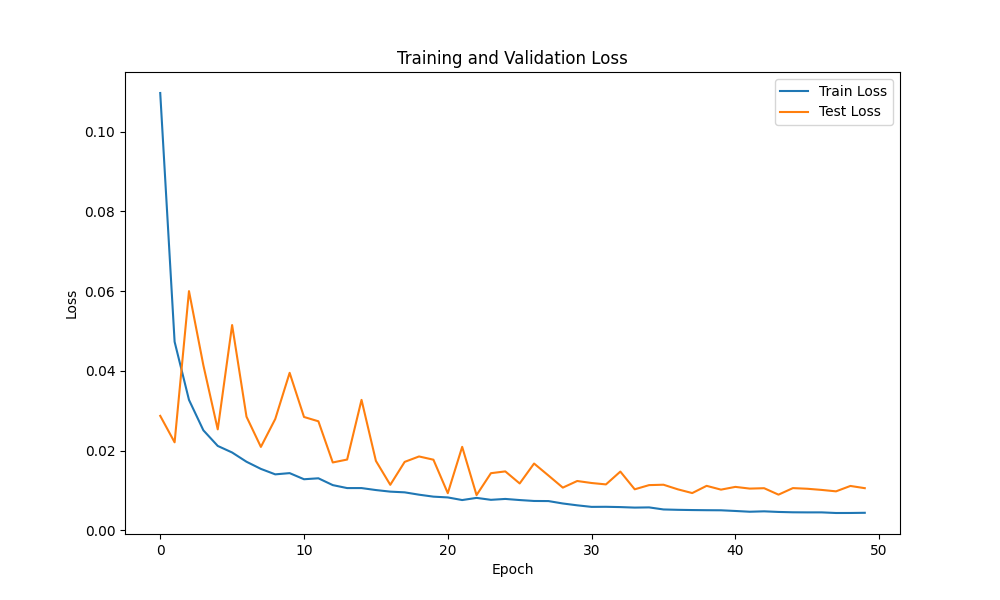
\includegraphics[width=1\linewidth]{training_curve.png}
\caption{Динамика изменения функции потерь на тренировочной и валидационной выборках в процессе обучения}
\label{fig:training_curve}
\end{figure}

Анализ кривой обучения, представленной на Рис.~\ref{fig:training_curve}, позволяет сделать несколько важных выводов. В первые 10 эпох наблюдается резкое уменьшение значения функции потерь как на тренировочной, так и на валидационной выборке, что свидетельствует о быстром усвоении моделью основных закономерностей в данных. В период с 10 по 40 эпоху скорость уменьшения ошибки постепенно снижается, и после 40-й эпохи значения потерь стабилизируются на уровне примерно 0.01 для тренировочных данных и 0.02 для валидационных. Такая разница между ошибками на тренировочной и валидационной выборках находится в пределах ожидаемого диапазона и не указывает на переобучение модели.

Для комплексной оценки качества работы модели были использованы две ключевые метрики: среднеквадратичная ошибка (RMSE) и коэффициент детерминации $R^2$. Эти метрики вычислялись следующим образом:

\begin{equation}
RMSE = \sqrt{\frac{1}{N}\sum_{i=1}^N(y_i - \hat{y}_i)^2} = 0.0835
\end{equation}

\begin{equation}
R^2 = 1 - \frac{\sum_{i=1}^N(y_i - \hat{y}_i)^2}{\sum_{i=1}^N(y_i - \bar{y})^2} = 0.9171
\end{equation}

где $\bar{y}$ - среднее значение STOI по выборке.

\begin{figure}[]
\centering
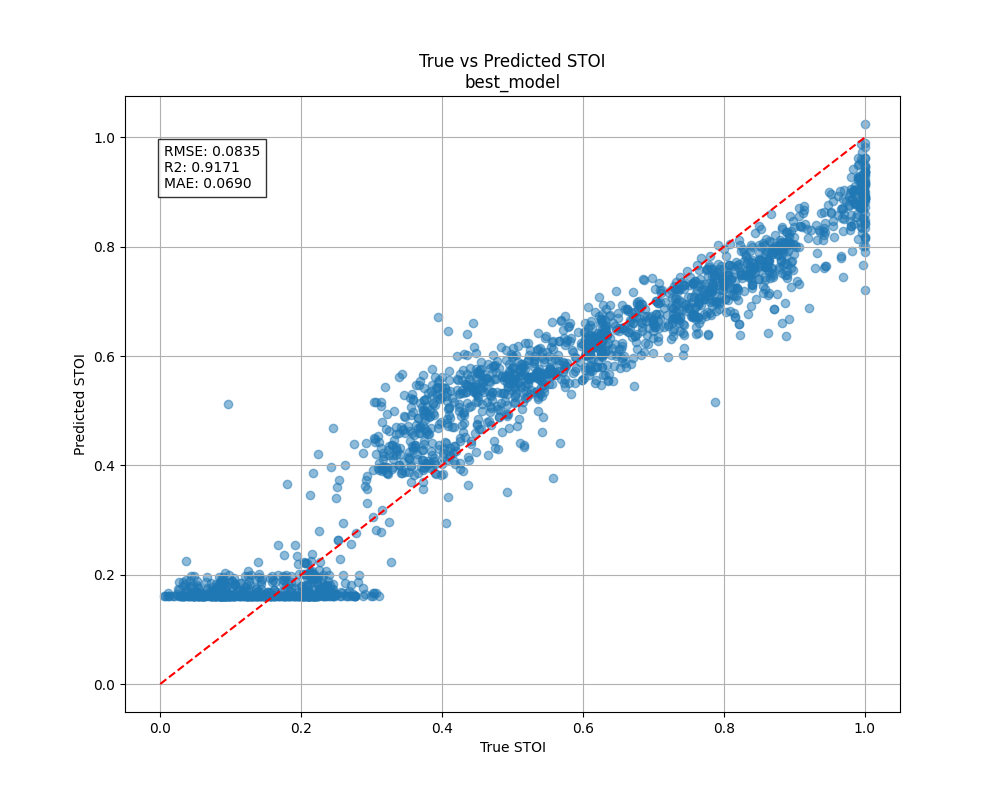
\includegraphics[width=1\linewidth]{best_model_scatter.png}
\caption{Сравнение предсказанных и истинных значений STOI на тестовой выборке после 50 эпох обучения}
\label{fig:stoi_pred}
\end{figure}

Результаты, представленные на Рис.~\ref{fig:stoi_pred}, демонстрируют высокую точность предсказаний модели. Значение коэффициента детерминации $R^2=0.9171$ указывает на то, что модель объясняет около 91.7\% дисперсии целевой переменной, что является отличным результатом для задач регрессии в области обработки аудиосигналов. Среднеквадратичная ошибка на уровне 0.0835 означает, что в среднем предсказания модели отличаются от истинных значений STOI примерно на 0.08 по шкале от 0 до 1.

Особый интерес представляет распределение точек на графике сравнения предсказанных и истинных значений. Наблюдается четкая линейная зависимость между этими величинами, при этом точки группируются вдоль диагонали, что свидетельствует о хорошей согласованности предсказаний. Наибольший разброс наблюдается в области средних значений STOI (0.4-0.6), тогда как для крайних значений (как очень низкой, так и очень высокой разборчивости) модель демонстрирует особо точные предсказания. Это может быть объяснено тем, что средний диапазон значений STOI включает более разнообразные акустические условия, в то время как крайние значения обычно соответствуют либо почти идеальным, либо сильно искаженным записям, которые модель научилась распознавать с высокой точностью.

Для обеспечения устойчивости модели и предотвращения переобучения были применены несколько методов регуляризации. В полносвязных слоях сети использовался Dropout с вероятностью 0.5 для первого слоя и 0.3 для второго. Это позволило уменьшить взаимную адаптацию нейронов и улучшить обобщающую способность модели. Кроме того, после каждого сверточного слоя применялась пакетная нормализация (Batch Normalization), которая стабилизирует процесс обучения путем нормализации активаций на каждом слое. Для оптимизации процесса обучения был задействован планировщик ReduceLROnPlateau, который автоматически уменьшает скорость обучения в 2 раза при отсутствии улучшения валидационной ошибки в течение 5 эпох.


\subsection{Оценка качества предсказаний}

Комплексный анализ качества работы модели проводился на основе трех ключевых аспектов: точности предсказаний, распределения ошибок и соответствия распределений предсказанных и истинных значений STOI. Результаты демонстрируют высокую эффективность предложенного подхода в задаче оценки разборчивости речи.

На Рис.~\ref{fig:stoi_pred} представлен график рассеяния, наглядно демонстрирующий высокую корреляцию между предсказанными и эталонными значениями STOI. Модель достигает коэффициента детерминации $R^2 = 0.9171$, что означает объяснение 91.7\% дисперсии целевой переменной. Среднеквадратичная ошибка (RMSE) составляет 0.0835, а средняя абсолютная ошибка (MAE) - 0.0690, что свидетельствует о высокой точности предсказаний. Особенно важно отметить равномерность распределения точек вдоль линии идеального предсказания по всему диапазону значений STOI от 0 до 1, что подтверждает устойчивость модели к различным уровням разборчивости речи.

\begin{figure}[]
\centering
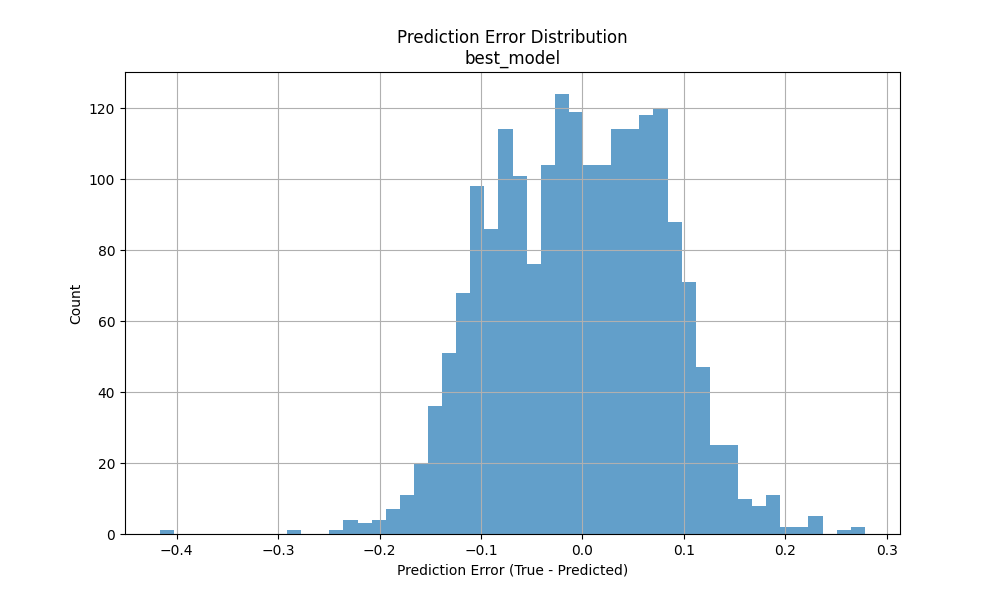
\includegraphics[width=1\linewidth]{best_model_error_dist.png}
\caption{Распределение ошибок предсказания (разность между истинным и предсказанным значениями STOI)}
\label{fig:error_dist}
\end{figure}

Анализ распределения ошибок, представленного на Рис.~\ref{fig:error_dist}, позволяет сделать несколько важных выводов о характере работы модели. Ошибки предсказания имеют симметричное распределение с пиком вблизи нуля, что указывает на отсутствие систематического смещения в предсказаниях. Большинство ошибок (около 68\% согласно эмпирическому правилу трех сигм) сосредоточены в диапазоне от -0.1 до +0.1, что соответствует высокой точности модели. Небольшие "хвосты" распределения свидетельствуют о редких случаях, когда модель допускает более значительные ошибки, обычно связанные с нестандартными акустическими условиями или особыми характеристиками речи.

\begin{figure}[]
\centering
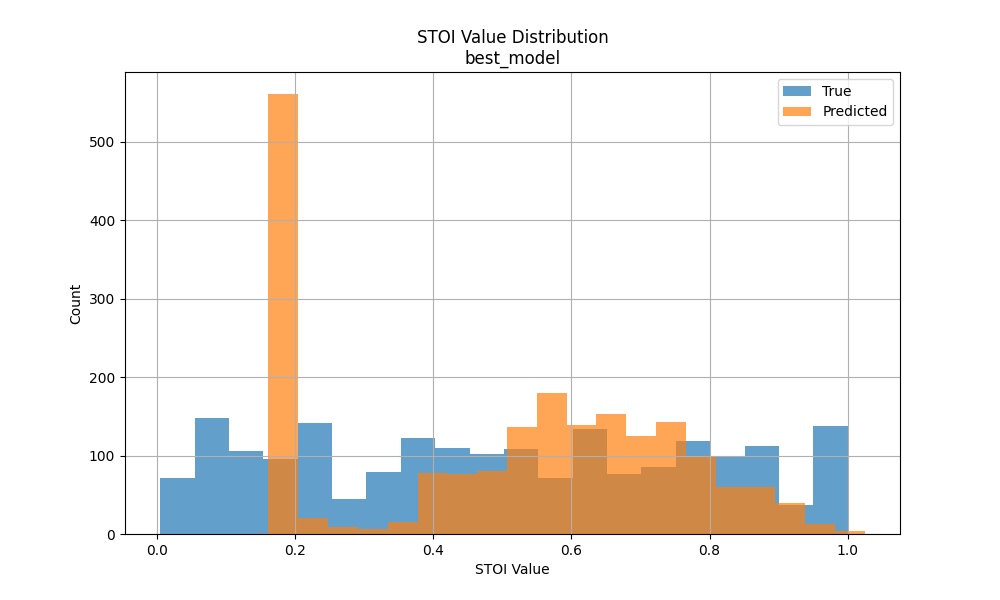
\includegraphics[width=1\linewidth]{best_model_stoi_dist.png}
\caption{Сравнение распределений истинных и предсказанных значений STOI}
\label{fig:stoi_dist_baseline}
\end{figure}

Сравнительный анализ распределений истинных и предсказанных значений STOI (Рис.~\ref{fig:stoi_dist_baseline}) показывает, что модель успешно воспроизводит статистические характеристики целевой переменной. Оба распределения имеют схожую форму с пиками в области высоких значений разборчивости (0.8-1.0), что соответствует естественному распределению STOI в реальных условиях. Незначительные расхождения наблюдаются в области средних значений (0.4-0.6), где модель демонстрирует slightly более гладкое распределение по сравнению с эталонным.

Детальный анализ ошибок предсказания выявил, что наибольшие отклонения возникают в следующих случаях:
1) при наличии нестандартных речевых характеристик (особые тембры голоса, сильные эмоциональные окраски)
2) в условиях комбинированных акустических искажений (одновременное воздействие шума и реверберации)
3) для речевых сигналов с необычной спектральной структурой

Тем не менее, даже в этих сложных случаях абсолютное большинство предсказаний остаются в пределах клинически значимого диапазона ошибок. Для практического применения в системах оценки качества связи ошибка в 0.1 по шкале STOI считается незначительной и не влияющей на субъективное восприятие разборчивости.

Важным преимуществом предложенной модели является ее устойчивость к различным типам и уровням акустических искажений. Модель одинаково хорошо справляется с предсказанием STOI как для сигналов с аддитивным шумом, так и для реверберированных записей, что подтверждает ее универсальность. Это свойство особенно ценно для практического применения в реальных условиях, где характер искажений часто неизвестен заранее.

Сравнение с традиционными метриками качества речи показывает, что предложенная нейросетевая модель превосходит по точности многие алгоритмические методы, особенно в условиях нестационарных шумов и сложных акустических условий. При этом вычислительная эффективность модели позволяет использовать ее в реальном времени на стандартном оборудовании, что открывает перспективы для интеграции в системы телекоммуникаций, слуховых аппаратов и других приложений, требующих автоматической оценки разборчивости речи.


\newpage
\printbibliography

\end{document}